\documentclass[aspectratio=169]{beamer}

% ---------- THEME & LOOK ----------
\usetheme{Madrid}
\usecolortheme{seahorse}
\usefonttheme{professionalfonts}
\setbeamertemplate{navigation symbols}{}
\setbeamercovered{transparent}
\setbeamertemplate{itemize items}[circle]
\setbeamertemplate{enumerate items}[default]
\setlength{\parskip}{0.25em}

% ---------- COLORS ----------
\usepackage{xcolor}
\definecolor{accent}{RGB}{0,92,184}
\setbeamercolor{structure}{fg=accent}
\setbeamercolor{title}{fg=white,bg=accent}
\setbeamercolor{frametitle}{fg=accent}
\setbeamercolor{block title}{bg=accent!10,fg=accent}
\setbeamercolor{block body}{bg=accent!3}

% ---------- PACKAGES ----------
\usepackage{booktabs}
\usepackage{amsmath, amssymb}
\usepackage{array}
\usepackage{hyperref}
\hypersetup{colorlinks=true,linkcolor=accent,urlcolor=accent}

% ---------- PLACEHOLDER BOX (compile-safe; no images required) ----------
\newcommand{\placeholderbox}[2][0.82\linewidth]{%
  \begin{center}
    \fbox{\begin{minipage}[c][0.46\textheight][c]{#1}
      \centering \vspace{0.25em}
      \textbf{#2}\\[0.6em]
      \emph{Insert figure/diagram here later.}
    \end{minipage}}
  \end{center}
}

% ---------- TITLE ----------
\title{\textbf{Labour Supply and Public Policy
 \vspace{.5cm}\\  }}
\subtitle{ {\large ECON 300 - Labour Economics}}
%\institute{UNBC}
\author{Muhebullah Karimzada}

\date{Winter 2026}

% ---------- SECTION INTRO SLIDES ----------
\AtBeginSection[]{
  \begin{frame}[plain]
    \transfade[duration=0.25]
    \centering
    {\usebeamerfont{title}\color{accent}\insertsectionhead}
    \vspace{0.8em}

    \begin{itemize}
      \item[] \textit{In this section we will:}
      \item<+-> Place each program into the income–leisure framework
      \item<+-> Compare work incentives via budget constraints
      \item<+-> Use diagrams (placeholders) you can fill later
    \end{itemize}
  \end{frame}
}

\begin{document}

% ============================================================
% TITLE
% ============================================================
\begin{frame}[plain]
  \titlepage
\end{frame}


\begin{frame}{Learning Objectives}
\transfade
\begin{itemize}
  \item Discuss key features of demogrants, social assistance, unemployment insurance, wage subsidies, workers’ compensation, and childcare subsidies.
  \item Use the labour supply model to analyze work incentives under demogrants, social assistance (with clawbacks), and wage subsidies.
  \item Analyze unemployment insurance within the income–leisure model and note empirical challenges.
  \item Graphically illustrate disability impacts on the budget constraint; compare compensation programs.
  \item Show how childcare costs and subsidies alter constraints and participation decisions.
\end{itemize}
\end{frame}

\begin{frame}{Main Questions}
\transfade
\begin{itemize}
  \item Can Canadian transfer programs be analyzed in a common framework to assess “best” designs for work incentives?
  \item Does unemployment insurance necessarily reduce incentives to work?
  \item Can welfare be designed to minimize adverse incentives while targeting need?
  \item How do we incorporate disabilities into the labour supply model and evaluate workers’ compensation?
  \item How do childcare costs and subsidies affect participation, hours, and the reservation wage?
\end{itemize}
\end{frame}


\begin{frame}{Income Maintenance Programs}
\transfade
\begin{itemize}
  \item Aim to supplement low incomes that arise for varied reasons; no single program fits all causes.
  \item Distinguish \textbf{permanent} (low wage) from \textbf{transitory} (hours shock) shortfalls—policy tools differ.
  \item \textbf{Universal} vs.\ \textbf{Targeted}: simplicity and coverage vs.\ cost and incentive effects.
\end{itemize}
\end{frame}

\begin{frame}{Universal vs.\ Targeted Programs}
\transfade
\begin{block}{Universal Programs}
Administratively simple; everyone receives the same transfer regardless of income. Expensive and benefits also flow to non-poor.
\end{block}
\begin{block}{Targeted Programs}
Cheaper: transfers top up to a threshold (e.g., poverty line) but can create \textbf{implicit taxes} on earnings that reduce work effort.
\end{block}
\end{frame}

\begin{frame}{TABLE 3.1: Government transfers received by Census Families in Canada, 2017}
\transfade
\small
\begin{tabular}{lcc}
\toprule
\textbf{Benefits} & \textbf{Percent of families} & \textbf{Average Amount} \\
\midrule
All government transfers (federal and provincial) & 83.7\% & \$12,750 \\
Federal Child Benefits & 20.2\% & \$6,314 \\
Provincial Child Benefits & 10.6\% & \$1,941 \\
Employment Insurance & 14.0\% & \$8,352 \\
Social Assistance & 11.3\% & \$8,367 \\
Workers’ Compensation & 3.5\% & \$9,820 \\
Canada/Quebec Pension Plan & 32.4\% & \$10,092 \\
Old Age Security & 25.1\% & \$8,566 \\
Guaranteed Income Supplement & 9.6\% & \$6,634 \\
\bottomrule
\end{tabular}
\end{frame}


\begin{frame}{Demogrants}
\transfade
\begin{itemize}
  \item Lump-sum transfer specific to a demographic group (e.g., OAS).
  \item \textbf{Work incentives:} No substitution effect; a pure \textbf{income effect} that tends to increase leisure and reduce hours.
  \end{itemize}
  \vspace{0.5cm}
\textbf{Note:} The income gain is partly “spent” on leisure, so income rises by less than the grant amount.

\end{frame}

\begin{frame}{Figure 3.1: Work Incentive Effects of a Lump-Sum Demogrant }
\centering
\vspace{2em}

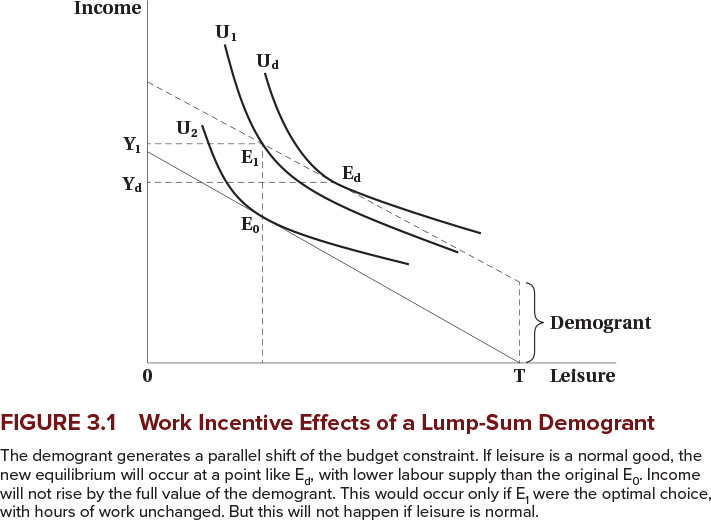
\includegraphics[width=0.77\linewidth]{ben54842_0301}.

\end{frame}

\begin{frame}{Welfare (Social Assistance)}
\transfade
\begin{itemize}
  \item Administered by provinces; partly financed by federal government.
  \item Benefits depend on need, assets, and other incomes.
\end{itemize}
\end{frame}

\begin{frame}{TABLE 3.2: Income of Welfare Recipients by Province, 2018 (lone parent, one child)}
\transfade
\small
\begin{tabular}{lcc}
\toprule
\textbf{Province} & \textbf{Annual Income\textsuperscript{a} (\$)} & \textbf{Income as \% of Poverty Line\textsuperscript{b}} \\
\midrule
Newfoundland & 23,436 & 85 \\
Prince Edward Island & 20,977 & 77 \\
Nova Scotia & 18,240 & 67 \\
New Brunswick & 19,978 & 78 \\
Quebec & 21,867 & 86 \\
Ontario & 21,463 & 72 \\
Manitoba & 21,764 & 82 \\
Saskatchewan & 21,087 & 77 \\
Alberta & 19,927 & 68 \\
British Columbia & 20,782 & 71 \\
\textbf{Average (unweighted)} & \textbf{20,952} & \textbf{76} \\
\bottomrule
\end{tabular}

\vspace{0.25em}
\scriptsize \textit{a.} Total annual income under program rules.\quad \textit{b.} Relative to poverty threshold used in the chapter.
\end{frame}

\begin{frame}{Figure 3.2: Work Incentive Effects of a Welfare Benefit with 100\% Clawback }
\centering
\vspace{2em}

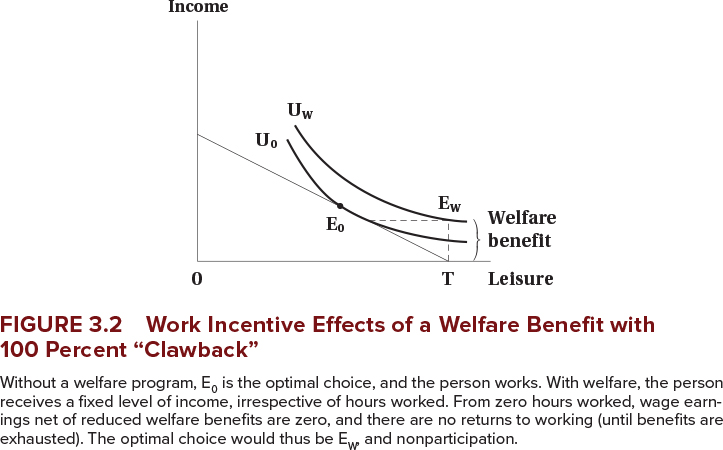
\includegraphics[width=0.98\linewidth]{ben54842_0302}.
\end{frame}

\begin{frame}{Improving Work Incentives in Welfare}
\transfade
\begin{itemize}
  \item Reduce the welfare benefit level (lower income effect).
  \item Raise the wage rate (tilt budget upward).
  \item Reduce the implicit tax rate (partial clawback).
  \item Shift preferences (e.g., work supports) toward market work.
\end{itemize}
\end{frame}

\begin{frame}{Figure 3.3: Other Work Incentive Effects of Welfare Programs }
\centering
\vspace{2em}

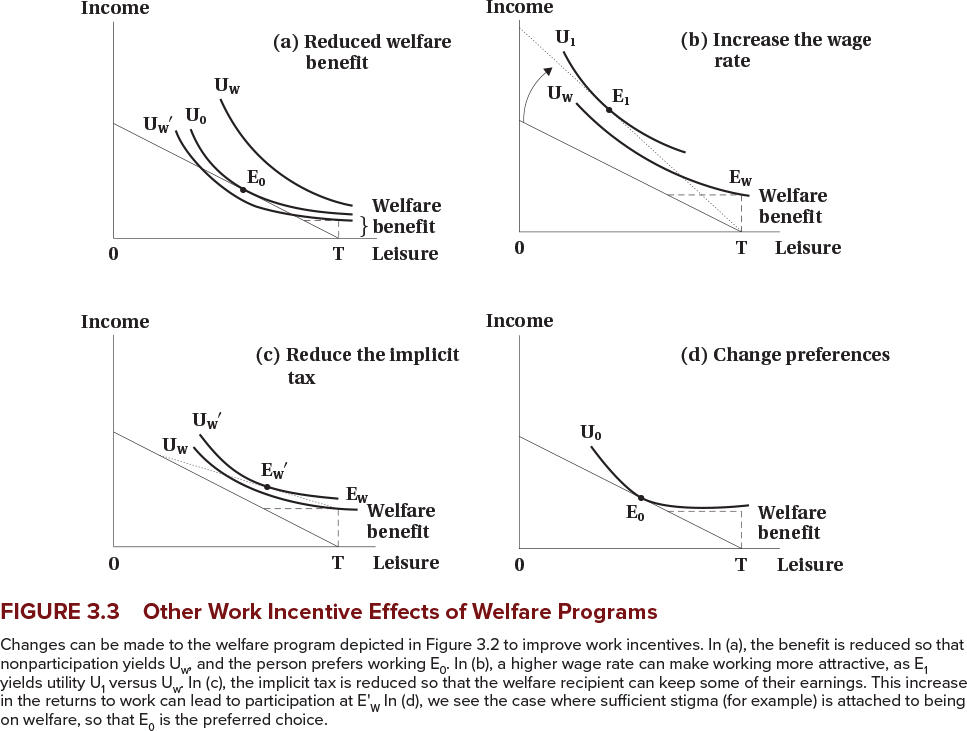
\includegraphics[width=0.72\linewidth]{ben54842_0303}.
\end{frame}

%\begin{frame}{Figure 3.4: Welfare Benefits, Beneficiaries, and Labour Market Conditions (Ontario)}
%\centering
%\vspace{2em}

%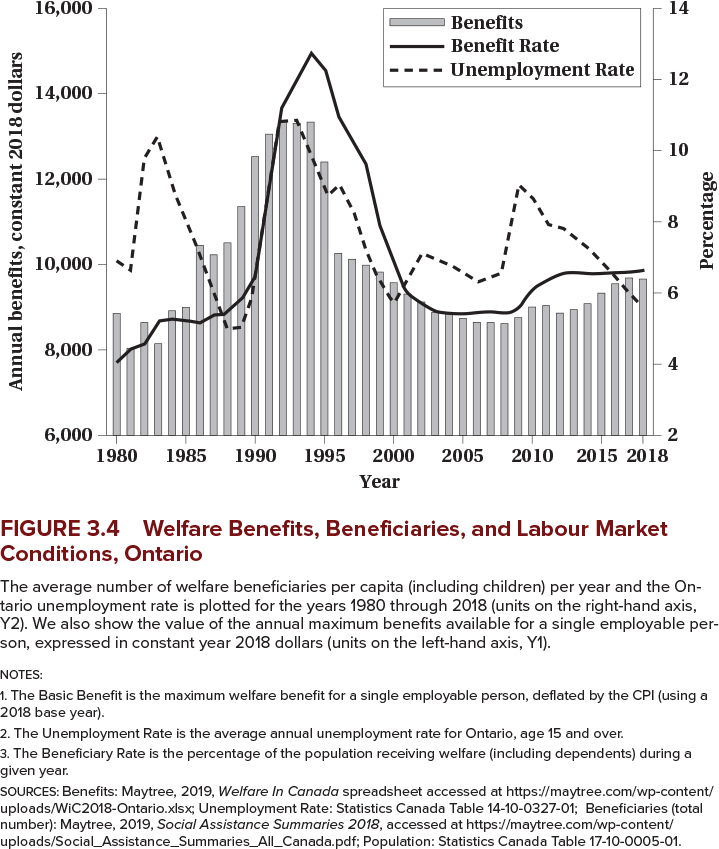
\includegraphics[width=0.62\linewidth]{ben54842_0304}.
%\end{frame}

\begin{frame}{Negative Income Tax (NIT)}
\transfade
\small
\textbf{Income guarantee with partial clawback:}
\[
Y = G + (1 - t)E
\]
\begin{itemize}
  \item \(G\): guaranteed income;\; \(t\): implicit tax rate;\; \(E\): earnings.
  \item Reduces hours via income effect and partial substitution effect (slope changes).
  \item Can replace welfare schemes with harsher disincentives.
\end{itemize}
\end{frame}

\begin{frame}{Figure 3.5: Work Incentive Effects of a Negative Income Tax }
\centering
\vspace{2em}

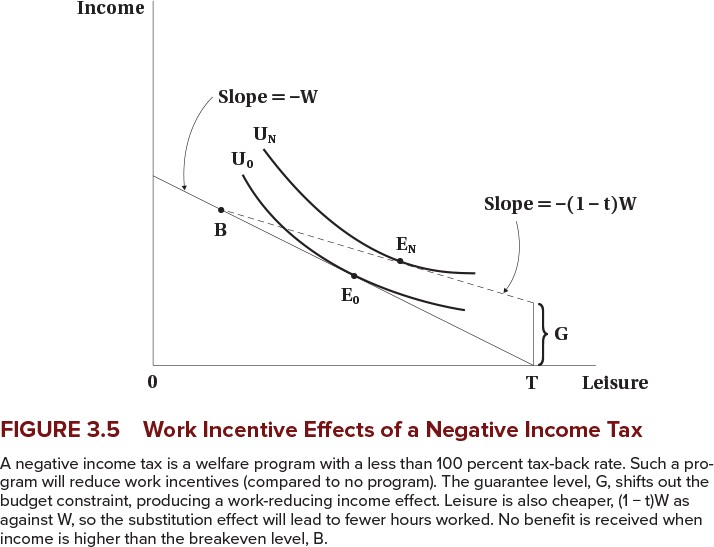
\includegraphics[width=0.76\linewidth]{ben54842_0305}.
\end{frame}

\begin{frame}{Wage Subsidy}
\transfade
\begin{itemize}
  \item Subsidizes earnings; raises effective wage.
  \item \textbf{Theoretical net effect on hours is indeterminate} (income vs.\ substitution work in opposite directions).
  \item Less adverse than a pure NIT for workers but does not help those unable to work.
\end{itemize}
\end{frame}

\begin{frame}{Figure 3.6: Work Incentive Effects of a Wage Subsidy }
\centering
\vspace{2em}

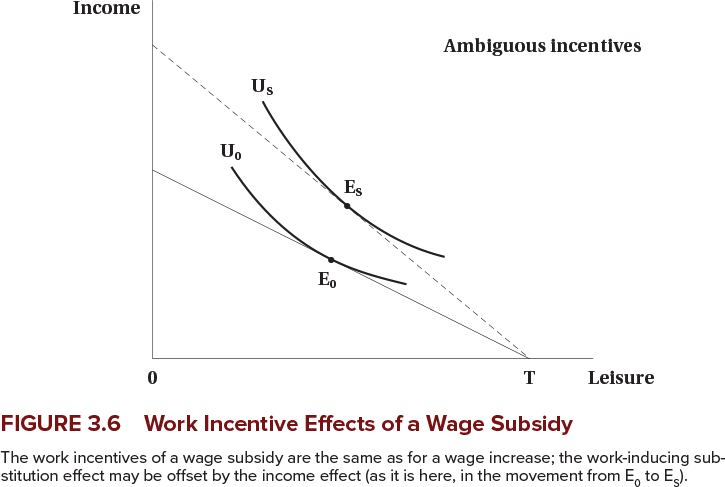
\includegraphics[width=0.82\linewidth]{ben54842_0306}.
\end{frame}

\begin{frame}{Refundable Tax Credit (Targeted Wage Subsidy)}
\transfade
\begin{itemize}
  \item Income-tested wage subsidy: \textbf{phase-in}, \textbf{flat}, and \textbf{phase-out} regions.
  \item Phase-in: substitution \(\uparrow\) (work more) vs.\ income \(\uparrow\) (work less) \(\Rightarrow\) ambiguous net.
  \item Flat: income effect only \(\Rightarrow\) hours fall (if leisure is normal).
  \item Phase-out: acts like NIT; substitution and income effects reduce work; participation effects can be clearer than hours.
\end{itemize}
\end{frame}

\begin{frame}{Figure 3.7: Work Incentives of a Refundable Tax Credit}
\centering
\vspace{2em}

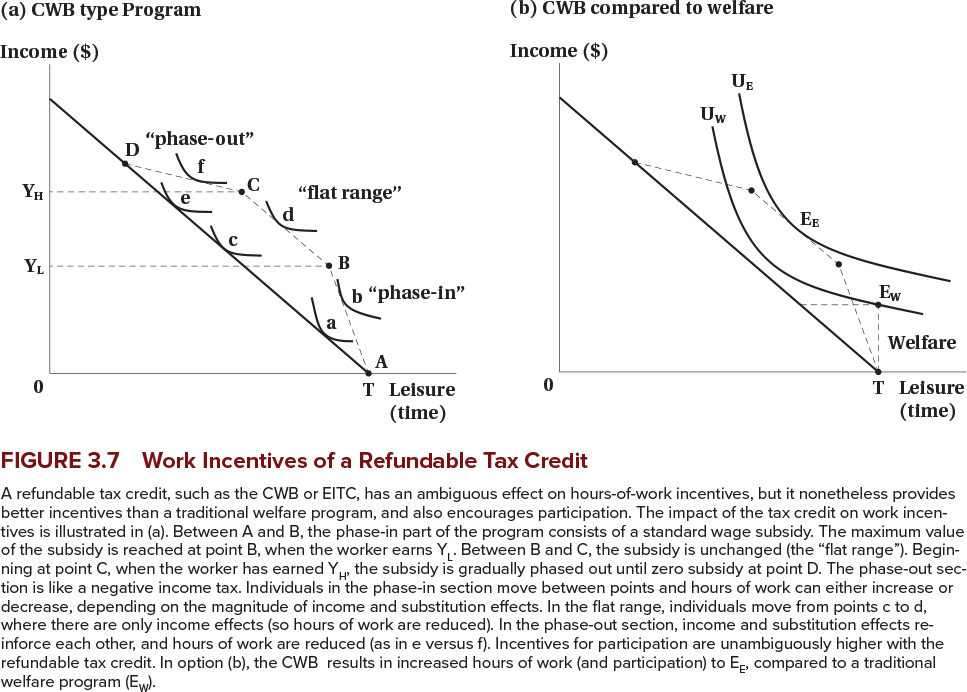
\includegraphics[width=0.955\linewidth]{ben54842_0307}.
\end{frame}


\begin{frame}{Unemployment Insurance (EI): Key Features}
\transfade
\begin{itemize}
  \item Largest income security program for non-elderly in Canada.
  \item Replacement rate \(\approx 55\%\) of lost earnings up to a maximum.
  \item Benefit duration: roughly 14–45 weeks, varying by local unemployment.
  \item Eligibility: roughly 420–700 hours worked (about 12–20 weeks at 35 hrs/week), depending on region.
\end{itemize}
\end{frame}

\begin{frame}{Worked Example: Unemployment Insurance and Work Incentives}
\transfade
\small
Suppose recipients receive 60\% of weekly pay if unemployed; must have worked at least 14 weeks to qualify; maximum benefit duration is 20 weeks.
\begin{itemize}
  \item \textbf{Income–leisure lens:} UI provides income when hours fall to zero, shifting choices along a non-linear budget across employment and non-employment states.
  \item \textbf{Predictions:} Longer/greater benefits \(\Rightarrow\) longer search duration; but also better job matching and consumption smoothing.
\end{itemize}
\end{frame}

\begin{frame}{Income Constraint for a Simplified Unemployment Insurance Scheme }
\centering
\vspace{2em}

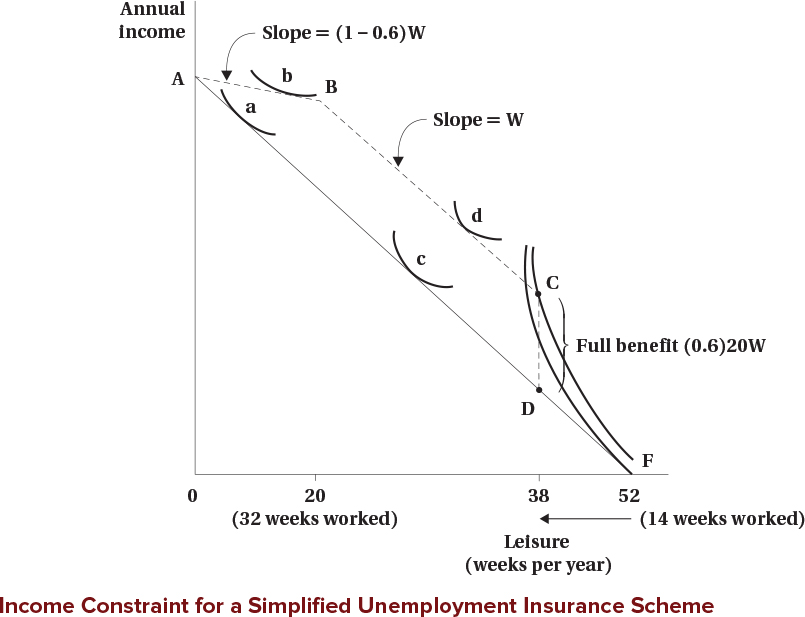
\includegraphics[width=0.61\linewidth]{ben54842_un0301}.
\end{frame}


\begin{frame}{Effect of a Disability}
\transfade
\begin{itemize}
  \item Alters budget (medical costs, fewer feasible hours) and/or preferences (higher disutility of work).
  \item Consider hours able to work, medical expenses, reduced wage-earning capacity, and relative disutility of market work.
\end{itemize}
\end{frame}

\begin{frame}{Figure 3.8: Effect of Disability }
\centering
\vspace{2em}

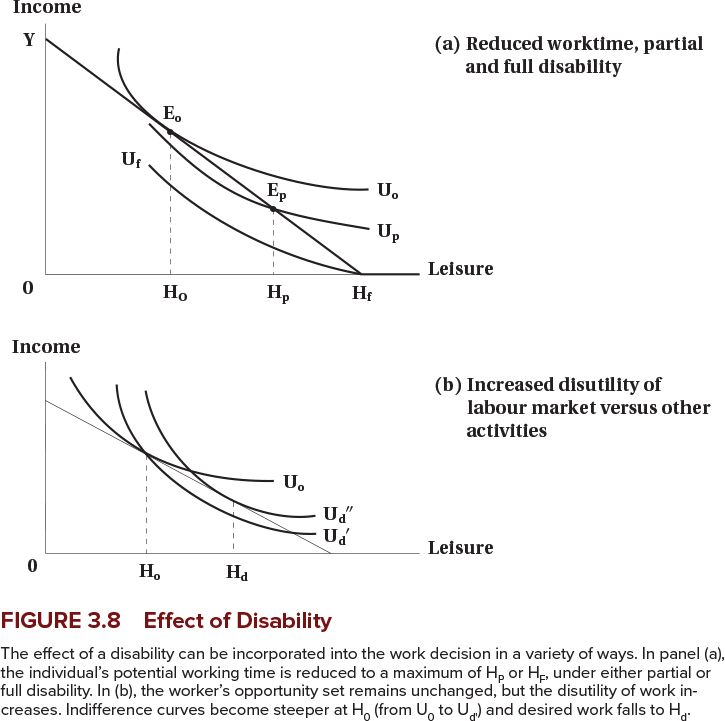
\includegraphics[width=0.55\linewidth]{ben54842_0308}.

\end{frame}

\begin{frame}{Figure 3.9: Effect of Compensation }
\centering
\vspace{2em}

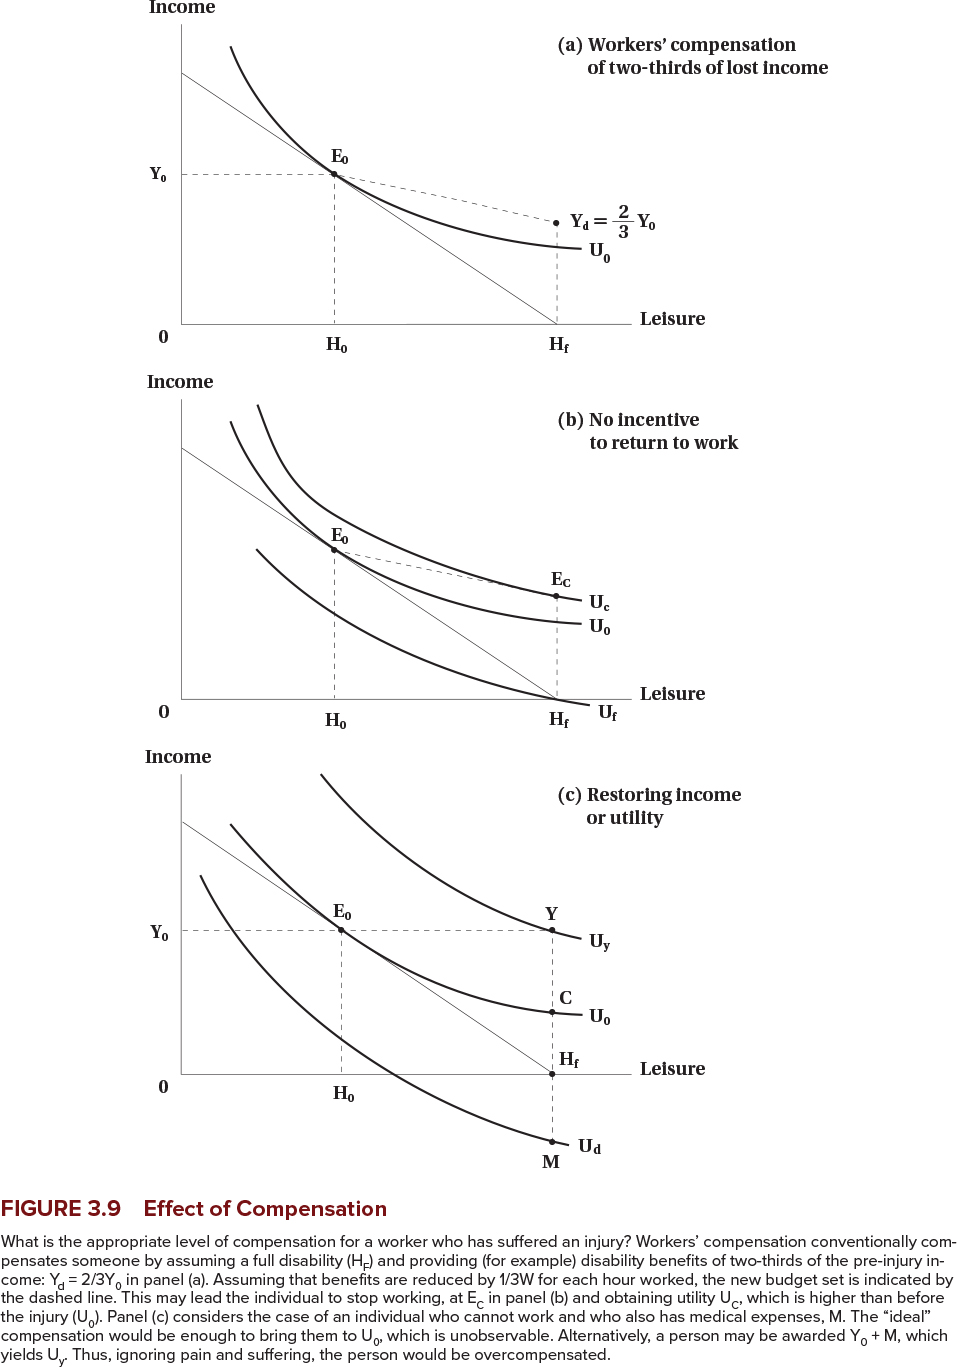
\includegraphics[width=0.363\linewidth]{ben54842_0309}.
\end{frame}


\begin{frame}{Child Care Costs and Subsidies}
\transfade
\begin{itemize}
  \item Daycare can be modeled as a \textbf{fixed cost of working}: reduces intercept or creates an entry “gap.”
  \item \textbf{Implications:} Raises reservation wage; can reduce hours for existing workers; can create non-convexities.
  \item Subsidies lower fixed cost, encouraging participation and part-time work; may reduce hours for some already working (income effect).
\end{itemize}
\end{frame}

\begin{frame}{Figure 3.10: The Effect of Child Care Costs on Labour Supply }
\centering
\vspace{2em}

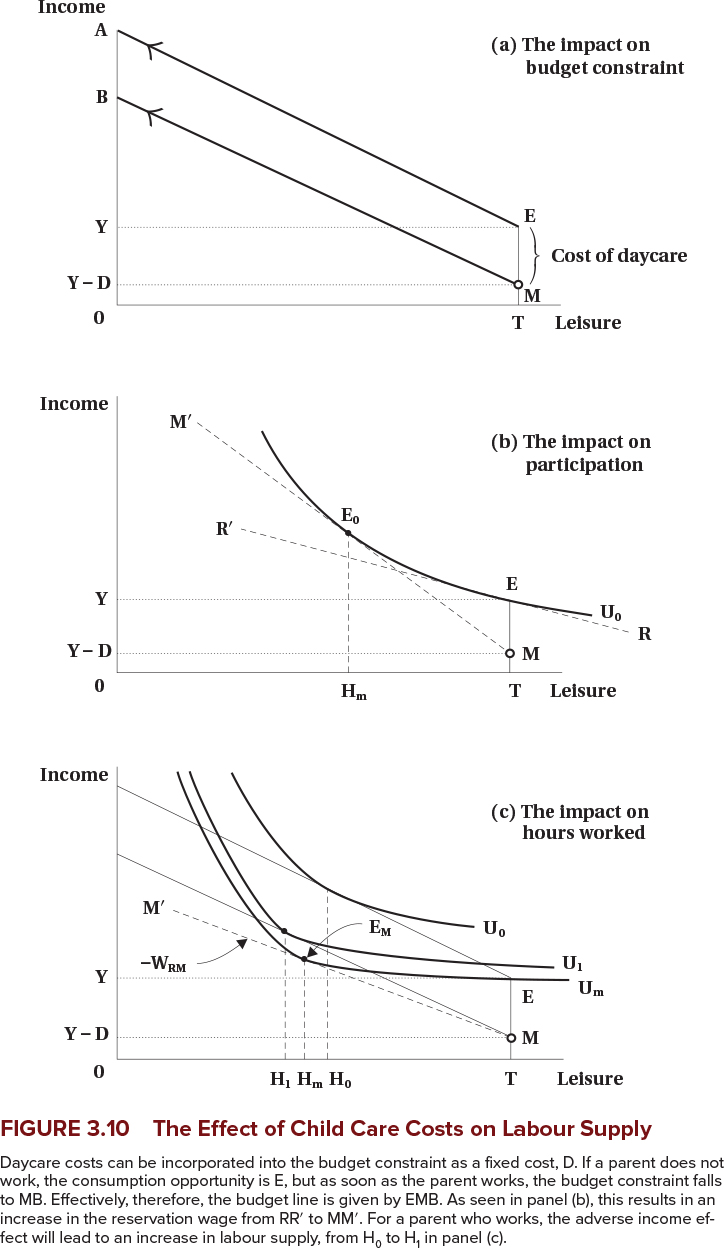
\includegraphics[width=0.29\linewidth]{ben54842_0310}.
\end{frame}


\begin{frame}{Summary (1/2)}
\transfade
\begin{itemize}
  \item Income maintenance schemes top up low incomes from varied causes; some are better for transitory shocks, others for persistent low wages.
  \item The labour supply framework compares work incentives across designs via their budget constraints.
  \item \textbf{Demogrants:} Pure income effect; reduce work incentives at the margin.
  \item \textbf{Welfare:} Adverse incentives magnified by high clawbacks; policy levers include earnings disregards and lower implicit tax rates.
\end{itemize}
\end{frame}

\begin{frame}{Summary (2/2)}
\transfade
\begin{itemize}
  \item \textbf{NIT:} Smoother guarantee with partial clawback; still reduces work relative to no transfer.
  \item \textbf{Wage Subsidies/Refundable Credits:} Encourage work on phase-in but can reduce hours on flat/phase-out; participation effects often clearer.
  \item \textbf{UI/EI:} Insures transitory hours shocks; trade-off between search/matching and potential work disincentives.
  \item \textbf{Disability/Workers’ Comp:} Shift constraints and preferences; evaluate well-being across program designs.
  \item \textbf{Childcare:} Fixed costs affect participation margins; subsidies can raise LFPR, especially for parents.
\end{itemize}
\end{frame}

% ============================================================
\begin{frame}
\centering
\Huge{\textbf{Thank You!}} \\

\end{frame}

\end{document}
